% Compile with XeLaTeX in TeXstudio.
% Notes: Some Word list paragraphs were mapped back to LaTeX headings.
% Review formulas, figure captions, and references before final thesis submission.

% Options for packages loaded elsewhere
\PassOptionsToPackage{unicode}{hyperref}
\PassOptionsToPackage{hyphens}{url}
%
\documentclass[
  a4paper,
]{report}
\usepackage{amsmath,amssymb}
\usepackage{iftex}
\ifPDFTeX
  \usepackage[T1]{fontenc}
  \usepackage[utf8]{inputenc}
  \usepackage{textcomp} % provide euro and other symbols
\else % if luatex or xetex
  \usepackage{unicode-math} % this also loads fontspec
  \defaultfontfeatures{Scale=MatchLowercase}
  \defaultfontfeatures[\rmfamily]{Ligatures=TeX,Scale=1}
\fi
\usepackage{lmodern}
\ifPDFTeX\else
  % xetex/luatex font selection
\fi
% Use upquote if available, for straight quotes in verbatim environments
\IfFileExists{upquote.sty}{\usepackage{upquote}}{}
\IfFileExists{microtype.sty}{% use microtype if available
  \usepackage[]{microtype}
  \UseMicrotypeSet[protrusion]{basicmath} % disable protrusion for tt fonts
}{}
\makeatletter
\@ifundefined{KOMAClassName}{% if non-KOMA class
  \IfFileExists{parskip.sty}{%
    \usepackage{parskip}
  }{% else
    \setlength{\parindent}{0pt}
    \setlength{\parskip}{6pt plus 2pt minus 1pt}}
}{% if KOMA class
  \KOMAoptions{parskip=half}}
\makeatother
\usepackage{xcolor}
\usepackage[margin=2.5cm]{geometry}
\usepackage{fontspec}
\usepackage{polyglossia}
\setmainlanguage{vietnamese}
\IfFontExistsTF{Times New Roman}{\setmainfont{Times New Roman}}{\setmainfont{DejaVu Serif}}
\usepackage{caption}
\usepackage{float}
\usepackage{longtable,booktabs,array}
\usepackage{calc} % for calculating minipage widths
% Correct order of tables after \paragraph or \subparagraph
\usepackage{etoolbox}
\makeatletter
\patchcmd\longtable{\par}{\if@noskipsec\mbox{}\fi\par}{}{}
\makeatother
% Allow footnotes in longtable head/foot
\IfFileExists{footnotehyper.sty}{\usepackage{footnotehyper}}{\usepackage{footnote}}
\makesavenoteenv{longtable}
\usepackage{graphicx}
\makeatletter
\def\maxwidth{\ifdim\Gin@nat@width>\linewidth\linewidth\else\Gin@nat@width\fi}
\def\maxheight{\ifdim\Gin@nat@height>\textheight\textheight\else\Gin@nat@height\fi}
\makeatother
% Scale images if necessary, so that they will not overflow the page
% margins by default, and it is still possible to overwrite the defaults
% using explicit options in \includegraphics[width, height, ...]{}
\setkeys{Gin}{width=\maxwidth,height=\maxheight,keepaspectratio}
% Set default figure placement to htbp
\makeatletter
\def\fps@figure{htbp}
\makeatother
\setlength{\emergencystretch}{3em} % prevent overfull lines
\providecommand{\tightlist}{%
  \setlength{\itemsep}{0pt}\setlength{\parskip}{0pt}}
% Đánh số tối đa đến \subsubsection, ví dụ 3.3.4.4.
% Các \paragraph bên dưới chỉ là tiêu đề nội bộ và không tạo cấp 3.3.4.4.x.
\setcounter{secnumdepth}{3}
\setcounter{tocdepth}{3}
\ifLuaTeX
  \usepackage{selnolig}  % disable illegal ligatures
\fi
\usepackage{bookmark}
\IfFileExists{xurl.sty}{\usepackage{xurl}}{} % add URL line breaks if available
\urlstyle{same}
\hypersetup{
  hidelinks,
  pdfcreator={LaTeX via pandoc}}

\title{Thiết kế hệ thống định vị thời gian thực sử dụng UWB}
\author{Phương}
\date{\today}

\begin{document}

\maketitle
\tableofcontents
\clearpage

\chapter{TỔNG QUAN}

\section{Lí do chọn đề tài}

\section{Mục tiêu nghiên cứu đề tài}

\section{Phương pháp nghiên cứu}

\section{Nội dung thực hiện}

\chapter{CƠ SỞ LÝ THUYẾT}

\section{Cơ sở lý thuyết về định vị}

\subsection{Khái niệm Ultra-Wideband}

\begin{quote}
Ultra-Wideband là công nghệ truyền thông vô tuyến sử dụng xung tín hiệu
có độ rộng rất ngắn trong miền thời gian, dẫn đến tín hiệu chiếm dụng
băng thông rất lớn trong miền tần số. Theo IEEE và FCC, một hệ thống
được phân loại là UWB khi băng thông chiếm dụng đạt tối thiểu
500~MHz~hoặc tương đương trên 20\% tần số trung tâm.~

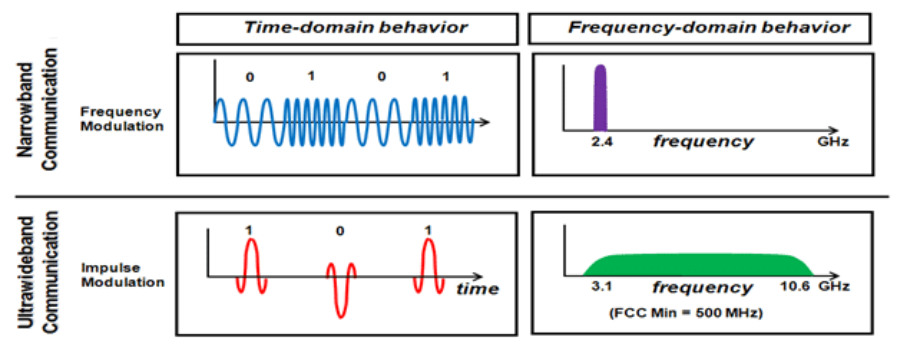
\includegraphics[width=6.2625in,height=2.48889in]{media/image1.png}Khác
với các hệ thống vô tuyến truyền thống (Wi-Fi,~Bluetooth), UWB không dựa
trên sóng mang liên tục để truyền dữ liệu. Thay vào đó, thông tin được
truyền bằng chuỗi xung ngắn, cho phép hệ thống làm việc chủ yếu trong
miền thời gian. Đây là nền tảng giúp UWB thực hiện đo thời gian lan
truyền sóng một cách trực tiếp.~

Hình 2.1. Bảng so sánh hình thái sóng trong miền thời gian và tần số
giữa UWB và các công nghệ định vị phổ biến
\end{quote}

\subsection{So sánh khả năng định vị của các công nghệ định vị hiện nay}

\subsection{Nguyên lý hoạt động và mô hình đo khoảng cách}

UWB khai thác trực tiếp khả năng~đo thời gian lan truyền của sóng vô
tuyến~ToF~để xác định khoảng cách giữa các thiết bị. Dựa~trên nguyên lý
cơ bản này, các hệ thống UWB có thể được triển khai theo nhiều mô hình
khác nhau nhằm đáp ứng các yêu cầu cụ thể về độ chính xác, quy mô mạng,
mức tiêu thụ năng lượng và độ phức tạp của hạ tầng.~

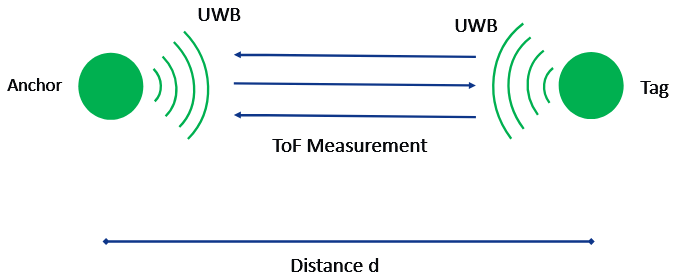
\includegraphics[width=5.70139in,height=2.36111in]{media/image2.png}Về
bản chất, mọi mô hình triển khai UWB đều dựa trên việc xác định mối quan
hệ thời gian giữa các tín hiệu phát và thu. Sự khác biệt giữa các mô
hình nằm ở cách tổ chức trao đổi gói tin, số lượng thiết bị tham gia đo,
cũng như mức độ đồng bộ thời gian cần thiết trong hệ thống.~

\subsubsection{Two-Way~Ranging~(TWR)~}

Two-Way~Ranging~là phương pháp đo khoảng cách dựa trên việc trao đổi gói
tin hai chiều giữa hai thiết bị UWB. Khoảng cách được suy ra từ thời
gian khứ hồi của tín hiệu, sau khi loại bỏ thời gian xử lý nội bộ của
thiết bị phản hồi.~

Ưu điểm cốt lõi của TWR là không yêu cầu đồng bộ tuyệt đối giữa đồng hồ
của hai thiết bị, giúp giảm đáng kể độ phức tạp phần cứng và phần mềm.
Tuy nhiên, tùy theo cách tổ chức trao đổi gói tin, TWR được chia thành
hai biến thể chính:~Single-Sided~TWR (SS-TWR) và~Double-Sided~TWR
(DS-TWR).~

\begin{itemize}
\item
  Single-Sided~Two-Way~Ranging~(SS-TWR)~
\end{itemize}

Trong SS-TWR, thiết bị khởi tạo (Initiator) gửi một gói tin đến thiết bị
phản hồi (Responder). Sau khi nhận được gói tin,~Responder~phản hồi lại
sau một khoảng thời gian xử lý cố định hoặc đã được cấu hình trước.~

Initiator~đo tổng thời gian khứ hồi của tín hiệu và trừ đi thời gian xử
lý của~Responder~để ước lượng thời gian lan truyền, từ đó tính toán
khoảng cách.~

Tuy nhiên, SS-TWR~\textbf{nhạy cảm với sai lệch~clock}~giữa hai thiết
bị. Nếu tần số~clock~của~Initiator~và~Responder~không ổn định hoặc bị
trôi, sai số đo có thể tăng đáng kể, đặc biệt trong các hệ thống yêu cầu
độ chính xác cao.~

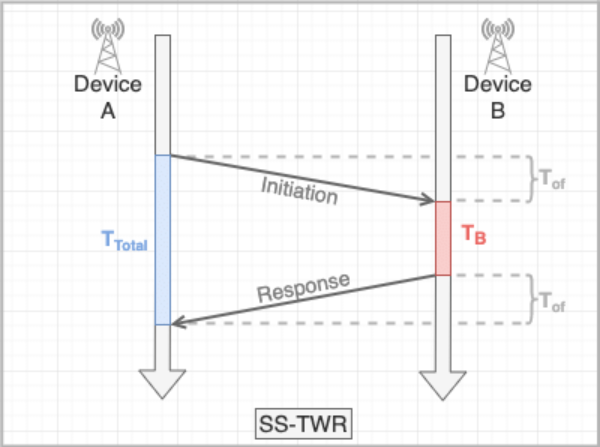
\includegraphics[width=4.16667in,height=3.10833in]{media/image3.png}~

\begin{itemize}
\item
  Double-Sided~Two-Way~Ranging~(DS-TWR)~
\end{itemize}

DS-TWR được phát triển nhằm khắc phục nhược điểm về sai lệch~clock~của
SS-TWR. Trong mô hình này, hai thiết bị trao đổi ít nhất ba gói tin, cho
phép cả hai bên cùng tham gia vào quá trình đo thời gian.~

Thông qua việc đo và trao đổi các~timestamp~ở cả hai phía, hệ thống có
thể~\textbf{bù trừ sai lệch~clock}~giữa các thiết bị, từ đó cải thiện
đáng kể độ chính xác của phép đo~ToF.~

\begin{quote}
Thông qua việc đo và trao đổi các~timestamp~ở cả hai phía, hệ thống có
thể~bù trừ sai lệch~clock~giữa các thiết bị, từ đó cải thiện đáng kể độ
chính xác của phép đo~ToF. Đổi lại là tăng số lượng gói tin và độ trễ,
với phương pháp thông thường thì cần khoảng \(3 \times N\) message với N
là số lượng anchor
\end{quote}

DS-TWR là phương pháp được sử dụng phổ biến trong các~chip~UWB
thương~mại, đặc biệt trong các ứng dụng định vị chính xác ở
mức~centimet.~

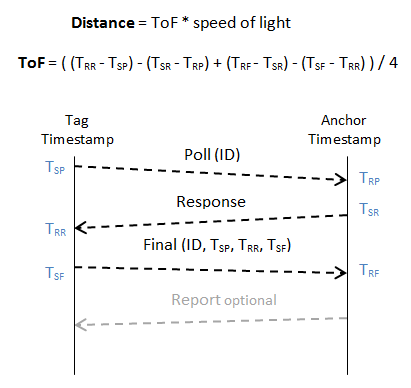
\includegraphics[width=3.42569in,height=3.23542in]{media/image4.png}\emph{Hình
2.4. Quy trình trao đổi gói tin với mô hình DS-TWR}

\subsubsection{Time~Difference~of~Arrival~(TDoA)~}

Time~Difference~of~Arrival~là mô hình triển khai UWB thường được sử dụng
trong các hệ thống định vị quy mô lớn với nhiều~anchor~cố định. Trong mô
hình này, thiết bị cần định vị (tag) phát một gói tin UWB, và
nhiều~anchor~thu tín hiệu đó gần như đồng thời.~

Thay vì đo thời gian lan truyền~tuyệt đối, hệ thống xác định sự chênh
lệch thời gian tín hiệu đến giữa các~anchor. Từ các sai khác này, vị trí
của~tag~được suy ra thông qua các thuật toán định vị dựa trên giao điểm
của các~hyperbol~thời gian.~

Điểm cốt lõi của~TDoA~là yêu cầu các~anchor~phải được~\textbf{đồng bộ
thời gian với độ chính xác rất cao}, thường thông qua đồng hồ chuẩn hoặc
mạng đồng bộ chuyên dụng. Cách~phổ~biến~nhất~là~dùng~một~Master
Anchor,~trong~đó~nó~sẽ~chủ~động~đồng~bộ~lại~thời~gian~với~các~Slave
Anchor.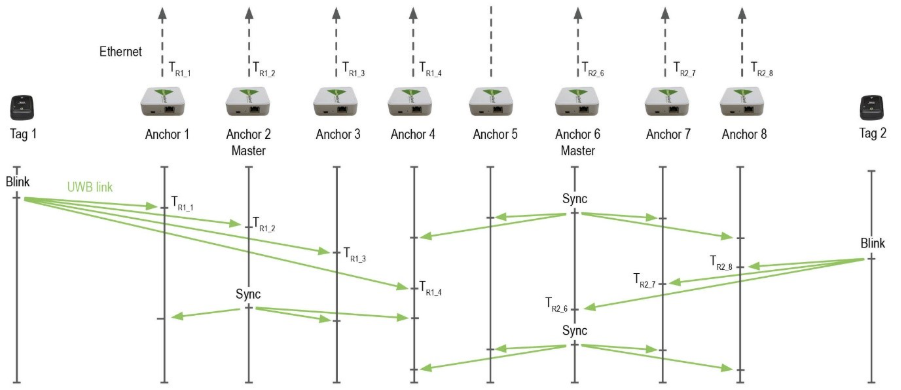
\includegraphics[width=6.25833in,height=2.70833in]{media/image5.png}~

\subsubsection{Phase~Difference~of~Arrival~(PDoA)~}

Phase~Difference~of~Arrival~là mô hình đo dựa trên~\textbf{sự chênh lệch
pha của tín hiệu UWB}~khi được thu tại các~anten~hoặc các điểm thu khác
nhau. Khoảng cách hoặc góc đến của tín hiệu được suy ra từ mối quan hệ
giữa pha tín hiệu và bước sóng.~

So với~ToF~hoặc~TDoA,~PDoA~\textbf{phụ thuộc mạnh vào đặc tính pha và
tần số}, do đó yêu cầu phần cứng có độ ổn định cao và hiệu chuẩn chính
xác. Do đó PDoA~ít phổ biến hơn TWR và~TDoA~trong các hệ thống UWB
thương mại, nhưng đóng vai trò quan trọng trong các giải pháp định vị
nâng cao.~

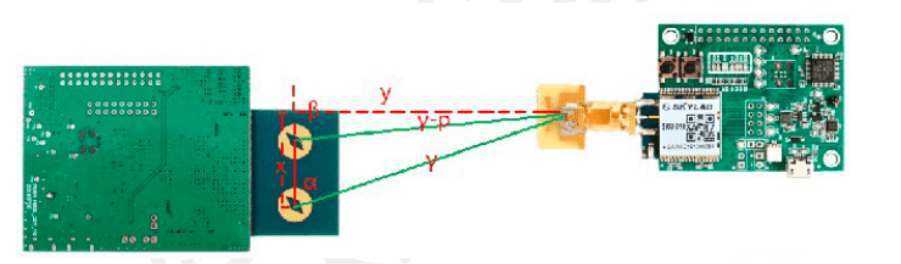
\includegraphics[width=6.25833in,height=1.83333in]{media/image6.png}

\subsection{Cơ chế truy nhập kênh và lập lịch truyền nhận trong hệ thống UWB nhiều anchor}

\subsubsection{Vai trò của lớp MAC trong hệ thống UWB nhiều anchor}

\begin{quote}
Trong hệ thống định vị UWB nhiều anchor, một tag cần đo khoảng cách với
nhiều anchor để thu thập đủ dữ liệu phục vụ quá trình ước lượng vị trí.
Với các phương pháp đo khoảng cách như DS-TWR, một phiên đo thường gồm
nhiều gói tin trao đổi theo trình tự, ví dụ Poll, Response và Final. Các
gói tin này được sử dụng để ghi nhận timestamp tại tag và anchor, từ đó
tính toán thời gian truyền tín hiệu.

Khi nhiều anchor hoặc nhiều tag cùng hoạt động trong một khu vực, các
thiết bị có thể phát sinh nhu cầu truyền nhận trong cùng thời điểm. Nếu
không có cơ chế điều phối, các gói tin có thể va chạm, làm mất timestamp
và khiến phiên đo khoảng cách không hợp lệ. Ngược lại, nếu các phiên đo
được thực hiện tuần tự nhưng không có lịch đo hợp lý, chu kỳ cập nhật vị
trí sẽ tăng khi số lượng anchor mở rộng. Vì vậy, lớp MAC được sử dụng để
điều phối quyền truy nhập kênh truyền, quy định thiết bị nào được
truyền, truyền vào thời điểm nào và sử dụng tài nguyên truyền thông nào.
\end{quote}

\subsubsection{Các nhóm cơ chế truy nhập kênh ở lớp MAC}

\begin{quote}
Các cơ chế đa truy nhập trong hệ thống truyền thông, hay Multiple Access
Protocols, được sử dụng để điều phối nhiều thiết bị cùng chia sẻ một môi
trường truyền dẫn. Các cơ chế này thường được phân thành ba nhóm chính:
truy nhập ngẫu nhiên, truy nhập có điều khiển và phân kênh.

Nhóm truy nhập ngẫu nhiên gồm các cơ chế như ALOHA, CSMA, CSMA/CD và
CSMA/CA, trong đó thiết bị chủ động quyết định thời điểm truyền và có
thể cần xử lý va chạm hoặc tránh va chạm.

Nhóm truy nhập có điều khiển gồm các cơ chế như reservation, polling và
token passing, trong đó quyền truyền được điều phối thông qua đặt trước
tài nguyên, thăm dò thiết bị hoặc truyền token.

Nhóm phân kênh gồm FDMA, TDMA và CDMA, trong đó tài nguyên truyền thông
được chia theo tần số, thời gian hoặc mã.

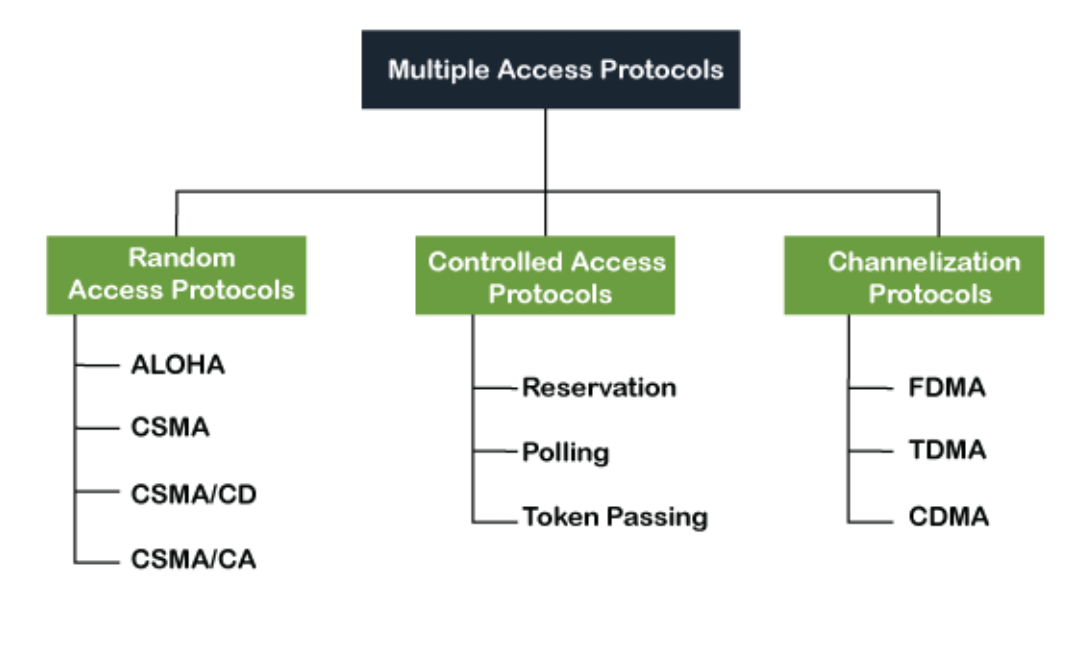
\includegraphics[width=5.56818in,height=3.34448in]{media/image7.png}
\end{quote}

Đối với hệ thống định vị UWB nhiều anchor sử dụng DS-TWR, yêu cầu quan
trọng là giảm va chạm gói tin và duy trì chu kỳ cập nhật vị trí ổn định.
Do đó, các cơ chế thuộc nhóm phân kênh phù hợp hơn cho luồng đo khoảng
cách chính, vì chúng cho phép tổ chức tài nguyên truyền nhận theo quy
tắc xác định. Trong phạm vi đề tài, TDMA được sử dụng để lập lịch các
phiên đo khoảng cách giữa tag và từng anchor theo các khe thời gian,
trong khi CDMA được xem xét thông qua việc sử dụng preamble code để phân
biệt hoặc phân nhóm tín hiệu giữa các anchor trong hệ thống UWB.

\subsubsection{TDMA trong lập lịch đo khoảng cách UWB}

TDMA là cơ chế phân chia truy nhập theo thời gian, trong đó quá trình
truyền nhận được chia thành các khe thời gian riêng biệt. Mỗi khe thời
gian được cấp cho một anchor, một tag hoặc một phiên đo cụ thể. Trong hệ
thống định vị UWB nhiều anchor, TDMA có thể được sử dụng để lập lịch cho
tag lần lượt đo khoảng cách với từng anchor theo một thứ tự xác định.

Ví dụ, trong một chu kỳ đo gồm bốn anchor, tag có thể thực hiện đo
khoảng cách với Anchor 1 ở khe thời gian thứ nhất, Anchor 2 ở khe thời
gian thứ hai, Anchor 3 ở khe thời gian thứ ba và Anchor 4 ở khe thời
gian thứ tư. Sau khi hoàn thành một chu kỳ TDMA, hệ thống thu được tập
dữ liệu khoảng cách từ tag đến các anchor để đưa vào thuật toán định vị.

Ưu điểm của TDMA là giảm khả năng va chạm gói tin và giúp hệ thống dự
đoán được thời gian hoàn thành một chu kỳ đo. Điều này đặc biệt quan
trọng đối với hệ thống định vị thời gian thực, vì chu kỳ đo ảnh hưởng
trực tiếp đến tần số cập nhật vị trí của xe tự hành. Tuy nhiên, khi số
lượng anchor tăng, tổng thời gian của một chu kỳ TDMA cũng tăng theo. Vì
vậy, việc lựa chọn số lượng anchor tham gia đo, độ dài khe thời gian và
thứ tự đo cần được thiết kế phù hợp với yêu cầu cập nhật vị trí của hệ
thống.

\subsubsection{CDMA và vai trò của preamble code trong UWB}

CDMA là cơ chế phân chia truy nhập theo mã, trong đó các tín hiệu được
phân biệt dựa trên mã khác nhau. Về nguyên lý, CDMA cho phép nhiều thiết
bị cùng sử dụng chung một dải tần, trong khi phía thu có thể phân biệt
tín hiệu dựa vào mã tương ứng. Trong các hệ thống UWB, cơ chế phân chia
theo mã có thể được nghiên cứu và ứng dụng để hỗ trợ nhiều node cùng
hoạt động trong một môi trường truyền thông.

Trong gói tin UWB, preamble là phần tín hiệu đầu gói được sử dụng để hỗ
trợ phát hiện gói tin, đồng bộ thời gian và nhận dạng tín hiệu ở phía
thu. Các thiết bị UWB có thể được cấu hình sử dụng các preamble code
khác nhau. Do đó, trong hệ thống nhiều anchor, preamble code có thể được
sử dụng như một cơ chế phân chia theo mã ở tầng vật lý, hỗ trợ phân biệt
tín hiệu giữa các node hoặc giữa các nhóm anchor khác nhau.

Trong phạm vi đề tài, CDMA được xem xét theo hướng sử dụng preamble code
để phân nhóm anchor. Cách tổ chức này cho phép các nhóm anchor được gán
các mã khác nhau, từ đó hỗ trợ quá trình nhận dạng tín hiệu và giảm ảnh
hưởng giữa các nhóm truyền thông UWB. Việc sử dụng preamble code không
thay thế vai trò lập lịch của TDMA, mà cung cấp thêm một chiều phân chia
tài nguyên theo mã bên cạnh phân chia theo thời gian.

Như vậy, TDMA và CDMA có thể được kết hợp trong hệ thống UWB nhiều
anchor. TDMA đảm nhiệm vai trò lập lịch thời điểm thực hiện các phiên đo
khoảng cách, trong khi CDMA thông qua preamble code hỗ trợ phân nhóm
anchor và phân biệt tín hiệu ở tầng vật lý. Sự kết hợp này giúp hệ thống
kiểm soát tốt hơn quá trình truyền nhận, hạn chế va chạm gói tin, duy
trì chu kỳ cập nhật ổn định và đáp ứng yêu cầu định vị thời gian thực
cho xe tự hành.

\section{Cơ sở thuật toán định vị thời gian thực}

\subsection{Thuật toán định vị hình học}

\subsubsection{Mô hình toán học của bài toán định vị theo khoảng cách}

Thuật toán định vị hình học là nhóm thuật toán sử dụng khoảng cách đo
được từ tag đến các anchor có tọa độ đã biết để ước lượng vị trí của
tag. Trong hệ thống định vị UWB, các khoảng cách này thường được thu từ
quá trình đo thời gian truyền tín hiệu giữa tag và anchor. Sau khi có dữ
liệu khoảng cách, bài toán định vị được chuyển thành bài toán hình học
trong mặt phẳng.

\begin{quote}
Gọi tọa độ của tag là \((x,y)\) và tọa độ của \(n\) anchor là
\(\left( x_{i},\ y_{i} \right).\) Khoảng cách đo được là \(d_{i}\). Khi
đó, trong điều kiện lý tưởng, vị trí của tag thỏa mãn phương trình:
\end{quote}

\begin{longtable}[]{@{}
  >{\raggedright\arraybackslash}p{(\columnwidth - 4\tabcolsep) * \real{0.0633}}
  >{\raggedright\arraybackslash}p{(\columnwidth - 4\tabcolsep) * \real{0.8615}}
  >{\raggedright\arraybackslash}p{(\columnwidth - 4\tabcolsep) * \real{0.0752}}@{}}
\toprule\noalign{}
\begin{minipage}[b]{\linewidth}\raggedright
\end{minipage} & \begin{minipage}[b]{\linewidth}\raggedright
\[\left( x - x_{i} \right)^{2} + \left( y - y_{i} \right)^{2} = d_{i}^{2}\]
\end{minipage} & \begin{minipage}[b]{\linewidth}\raggedright
(2.1)
\end{minipage} \\
\midrule\noalign{}
\endhead
\bottomrule\noalign{}
\endlastfoot
\end{longtable}

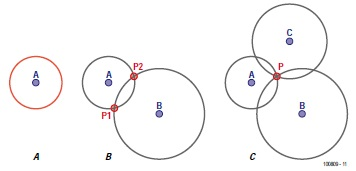
\includegraphics[width=4.72917in,height=2.27569in]{media/image8.jpeg}Phương
trình trên biểu diễn một đường tròn có tâm tại anchor \(A_{i}\) và bán
kính bằng khoảng cách đo được di. Vì vậy, về mặt hình học, vị trí của
tag có thể được xác định từ giao điểm của các đường tròn khoảng cách.
Trong trường hợp lý tưởng, các đường tròn này giao nhau tại đúng vị trí
thật của tag. Tuy nhiên, trong thực tế, dữ liệu đo luôn tồn tại sai số
nên các đường tròn có thể không giao nhau chính xác tại một điểm.

Hình 2.5. Mô hình xác định vị trí dựa trên giao điểm của các đường tròn

\subsubsection{Phương pháp trilateration}

Trilateration là phương pháp xác định vị trí từ khoảng cách đến các điểm tham
chiếu có tọa độ đã biết. Trong bài toán hai chiều, mỗi phép đo khoảng cách xác
định một đường tròn có tâm tại anchor và bán kính bằng khoảng cách đo. Với ba
anchor không thẳng hàng, vị trí của tag được xác định từ giao điểm của ba
đường tròn trong trường hợp lý tưởng.

Trilateration có ưu điểm là mô hình đơn giản, số phép đo yêu cầu ít và phù hợp
với các hệ thống có tài nguyên tính toán hạn chế. Tuy nhiên, phương pháp phụ
thuộc mạnh vào chất lượng từng khoảng cách và cách bố trí anchor. Khi các
anchor gần thẳng hàng, một sai lệch nhỏ của khoảng cách có thể tạo ra sai lệch
lớn của vị trí. Trong môi trường có nhiễu, các đường tròn thường không giao
nhau tại cùng một điểm nên cần sử dụng nghiệm xấp xỉ.

\begin{figure}[H]
  \centering
  \fbox{\parbox[c][4cm][c]{0.78\linewidth}{\centering
  Vị trí chèn hình minh họa trilateration với ba đường tròn khoảng cách}}
  \caption{Nguyên lý xác định vị trí bằng trilateration.}
  \label{fig:trilateration-concept}
\end{figure}

\subsubsection{Phương pháp multilateration}

Multilateration mở rộng trilateration bằng cách sử dụng nhiều hơn số phép đo
tối thiểu. Khi có $N>3$ anchor trong bài toán hai chiều, hệ thống thu được một
hệ phương trình dư. Vị trí không còn được xác định bằng một giao điểm hình học
duy nhất mà bằng nghiệm phù hợp nhất với toàn bộ tập khoảng cách.

Thông tin dư giúp giảm sự phụ thuộc vào một anchor riêng lẻ, cho phép phát
hiện phép đo không nhất quán và cải thiện độ ổn định của nghiệm. Đổi lại,
multilateration cần một tiêu chuẩn tối ưu để phân phối ảnh hưởng của các phép
đo. Bình phương tối thiểu xem các phép đo có độ tin cậy tương đương, trong khi
bình phương tối thiểu có trọng số cho phép mỗi khoảng cách đóng góp khác nhau
tùy theo phương sai hoặc chất lượng quan sát.

Hiệu quả của multilateration vẫn phụ thuộc vào hình học anchor. Việc tăng số
anchor không bảo đảm tăng độ chính xác nếu các anchor tập trung trên cùng một
hướng hoặc nếu các phép đo bổ sung có sai lệch hệ thống. Vì vậy, số lượng,
chất lượng phép đo và độ phân tán hình học cần được xem xét đồng thời.

\begin{figure}[H]
  \centering
  \fbox{\parbox[c][4cm][c]{0.78\linewidth}{\centering
  Vị trí chèn hình minh họa multilateration với hệ đường tròn dư}}
  \caption{Nguyên lý ước lượng vị trí bằng multilateration.}
  \label{fig:multilateration-concept}
\end{figure}

\subsection{Đánh giá sai số và độ tin cậy của kết quả định vị}

Khoảng cách UWB đo được không chỉ chứa khoảng cách hình học thực mà còn chịu
ảnh hưởng của nhiễu ngẫu nhiên và sai lệch có hệ thống. Một mô hình khái quát
cho phép đo thứ $i$ là
\begin{equation}
  d_i=\rho_i+b_i+\varepsilon_i,
  \label{eq:ranging-error-model}
\end{equation}
trong đó $\rho_i$ là khoảng cách thực, $b_i$ là thành phần sai lệch và
$\varepsilon_i$ là nhiễu ngẫu nhiên. Trong điều kiện LOS thuận lợi,
$b_i$ thường nhỏ; trong điều kiện NLOS hoặc đa đường, thành phần này có thể
tăng đáng kể và thường mang dấu dương do đường truyền bị kéo dài.

Độ tin cậy của một phép đo cần được xem xét từ nhiều nguồn thông tin. Sai số
dư cho biết mức phù hợp giữa một khoảng cách và nghiệm vị trí hình học. Tuy
nhiên, residual không đồng nhất với sai số thực: một tập phép đo cùng bị lệch
vẫn có thể tạo residual nhỏ. Do đó residual cần được diễn giải cùng với đặc
tính thống kê và điều kiện thu tín hiệu.

Khoảng cách Mahalanobis là thước đo sai lệch có chuẩn hóa theo hiệp phương
sai. Khác với khoảng cách Euclid, đại lượng này xét cả độ lớn, độ phân tán và
tương quan giữa các biến quan sát. Vì vậy, nó phù hợp để xác định một mẫu có
nằm trong vùng phân bố thông thường hay không, đặc biệt khi các đặc trưng có
đơn vị và độ biến thiên khác nhau.

Các chỉ số chất lượng tín hiệu như biên độ đường truyền đầu tiên, công suất
thu, tỷ số tín hiệu trên nhiễu và dấu hiệu NLOS phản ánh điều kiện lan truyền
nhưng không trực tiếp đồng nhất với sai số khoảng cách. Quan hệ giữa chúng
thường phụ thuộc phần cứng, anten, khoảng cách và môi trường, do đó cần được
đặc trưng bằng dữ liệu đo thay vì sử dụng một ngưỡng chung cho mọi điều kiện.

Bên cạnh chất lượng từng phép đo, hình học anchor quyết định khả năng biến đổi
sai số khoảng cách thành sai số tọa độ. Các đường ngắm phân bố trên nhiều
hướng tạo điều kiện quan sát tốt; cấu hình gần thẳng hàng hoặc tập trung về
một phía làm bài toán kém điều kiện. Vì vậy, độ tin cậy của kết quả vị trí là
tổng hợp của sai số đo, mức bất định thống kê và hình học của toàn bộ tập
anchor.

\subsection{Bộ lọc Unscented Kalman Filter trong hệ thống định vị UWB--IMU}

UKF là bộ lọc trạng thái phi tuyến sử dụng tập sigma point để xấp xỉ sự lan
truyền của trung bình và hiệp phương sai qua mô hình động học và mô hình đo.
Trong hệ thống UWB--IMU, UKF cho phép duy trì quỹ đạo liên tục, kết hợp thông
tin chuyển động với khoảng cách UWB và dự đoán ngắn hạn khi một số phép đo
tạm thời không hợp lệ.
\section{Cơ sở thiết kế mạch định vị}

\section{Cơ sở lý thuyết về truyền thông và phần mềm cho hệ thống định vị UWB}

\begin{enumerate}
\def\labelenumi{\arabic{enumi}.}
\item
  Vai trò của khối truyền thông trong hệ thống định vị UWB
\item
  BLE, \ldots{}
\item
  Protobuf, \ldots{}
\item
  Hệ điều hành thời gian thực cho hệ thống nhúng
\end{enumerate}

\chapter{THIẾT KẾ HỆ THỐNG ĐỊNH VỊ THỜI GIAN THỰC}

\section{Tổng quan kiến trúc hệ thống định vị}

\subsection{Thành phần và mô hình triển khai hệ thống}

\subsection{Luồng dữ liệu và điều khiển tổng thể}

\section{Thiết kế phần cứng và lựa chọn linh kiện cho bo mạch}

\subsection{Sơ đồ khối phần cứng tổng thể của hệ thống định vị}

\subsection{Tính toán và lựa chọn linh kiện}

\subsubsection{Tính toán dung lượng pin và ước tính thời gian sạc}

\subsubsection{Tính toán xung nhịp hệ thống và giá trị thạch anh}

\subsubsection{Thiết kế và lựa chọn linh kiện cho khối nguồn}

\subsubsection{Thiết kế khối điều khiển}

\subsection{Thiết kế mạch in PCB}

\subsubsection{Đặc tính vật lý và cấu trúc lớp}

\subsubsection{Tính toán và thiết lập độ rộng đường dây}

\subsubsection{Thiết lập quy chuẩn lỗ xuyên}

\subsubsection{Sơ đồ đi dây và bố trí linh kiện}

\subsubsection{Mạch in 3D}

\subsection{Thiết kế vỏ hộp 3D}

\subsection{Lắp ráp, kiểm tra và thử nghiệm phần cứng}

\section{Thiết kế và triển khai firmware vi điều khiển trung tâm}

\subsection{Phân bổ không gian bộ nhớ hệ thống và cấu trúc lưu trữ dữ liệu}

Vi điều khiển trung tâm cung cấp 512 KB bộ nhớ Flash và 128 KB
SRAM\ldots.

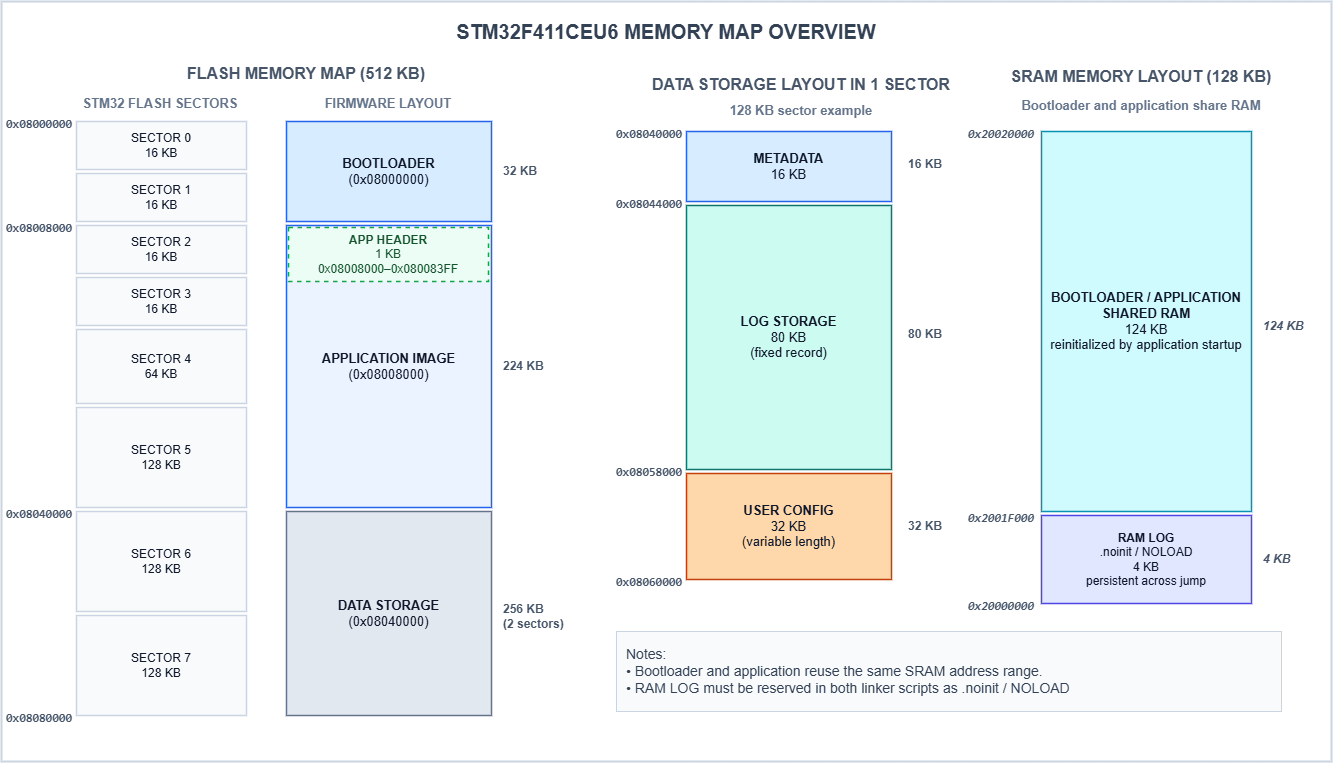
\includegraphics[width=6.5in,height=3.71944in]{media/image9.png}

\subsubsection{\textbf{Phân bổ vùng trong bộ nhớ Flash}}

Bộ nhớ Flash được chia thành ba vùng độc lập: bootloader, firmware ứng
dụng và dữ liệu lưu trữ. Ranh giới giữa các vùng được xác định trong
linker script nhằm ngăn chương trình hoặc thao tác cập nhật truy cập
ngoài phạm vi được cấp phát.

\textbf{Vùng bootloader:} chiếm 48 KB đầu tiên của Flash và chứa chương
trình khởi động, xác thực và nâng cấp firmware.

\textbf{Vùng ứng dụng:} bắt đầu tại địa chỉ 0x0800C000 với dung lượng
208 KB. Trong đó, 1 KB đầu được dành cho bảng vector và tiêu đề ảnh;
phần còn lại chứa chương trình ứng dụng.

\textbf{Vùng lưu trữ:} chiếm 256 KB cuối của Flash và gồm hai sector có
dung lượng bằng nhau. Vùng này lưu cấu hình, metadata và nhật ký vận
hành, đồng thời hỗ trợ cơ chế wear-leveling được trình bày tại Mục
3.2.1.3.

\subsubsection{Phân bổ vùng trong bộ nhớ RAM}

SRAM được chia thành vùng làm việc thông thường và vùng dùng chung. Do
bootloader và ứng dụng không thực thi đồng thời, hai chương trình có thể
tái sử dụng cùng vùng RAM để lưu biến, stack, heap, bộ đệm và các đối
tượng FreeRTOS.

Phần cuối SRAM được dành cho vùng NOLOAD, có nội dung không bị khởi tạo
lại khi chuyển từ bootloader sang ứng dụng. Vùng này lưu nhật ký chẩn
đoán và thông tin bàn giao qua reset mềm. Tuy nhiên, dữ liệu không được
duy trì khi thiết bị mất nguồn nên không thay thế cho vùng lưu trữ trong
Flash.

\subsubsection{Vùng lưu trữ và nguyên lý wear-leveling}

Flash chỉ có thể ghi vào vùng đã được xóa, trong khi thao tác xóa được
thực hiện trên toàn bộ sector. Nếu cấu hình và nhật ký chỉ được lưu
trong một sector, các lần cập nhật liên tục sẽ làm số chu kỳ xóa tập
trung tại sector đó. Vì vậy, hệ thống sử dụng hai sector và luân phiên
vai trò giữa chúng nhằm phân bố số lần xóa.

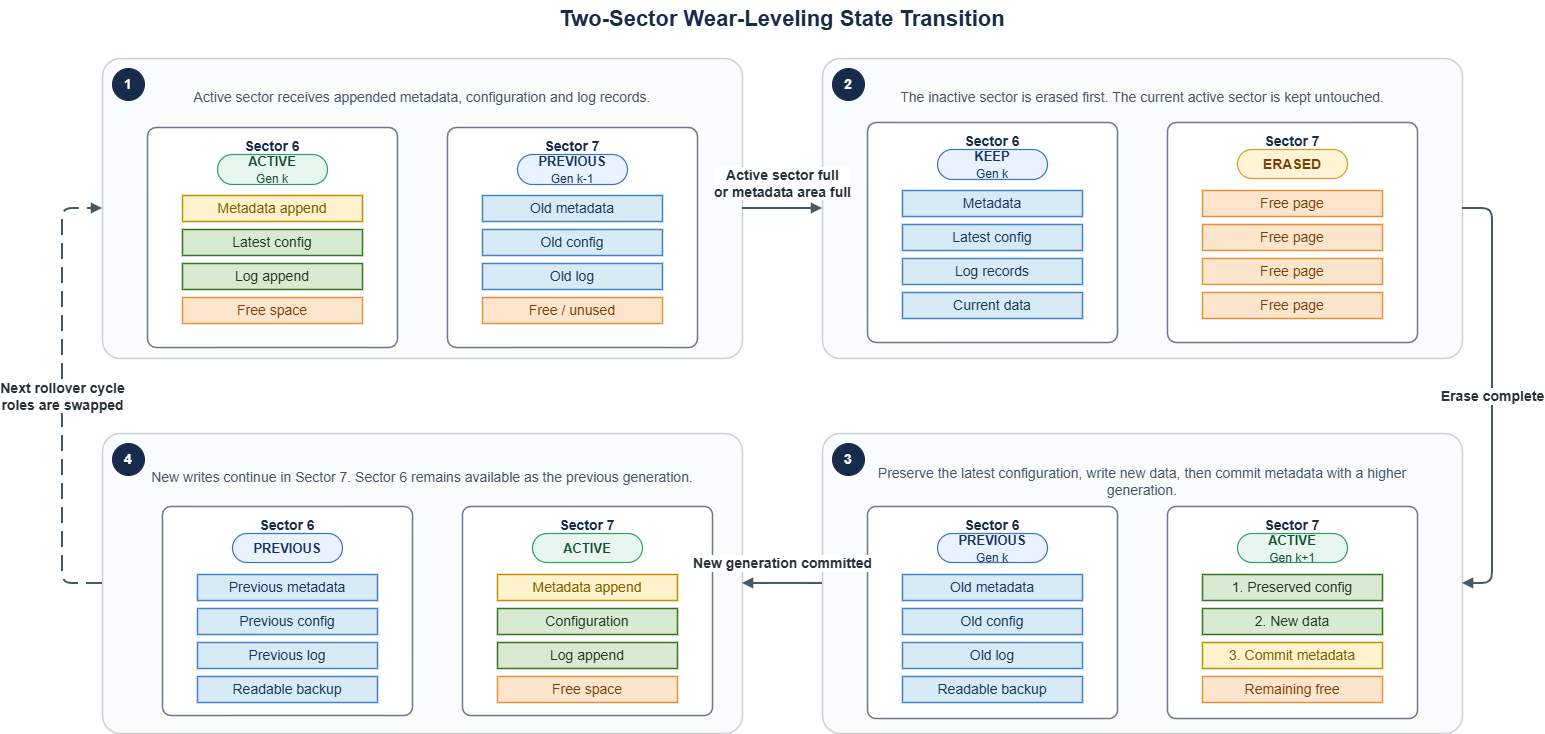
\includegraphics[width=6.79839in,height=3.23214in]{media/image10.png}Tại
một thời điểm, một sector giữ vai trò hoạt động và tiếp nhận các bản ghi
mới. Sector còn lại lưu dữ liệu của thế hệ trước hoặc chờ được tái sử
dụng. Khi sector hoạt động không còn đủ không gian, hệ thống xóa sector
còn lại, chuyển dữ liệu cần bảo toàn sang đó và tăng số generation. Sau
khi quá trình ghi hoàn tất, sector mới trở thành sector hoạt động, còn
sector cũ được giữ nguyên cho đến lần chuyển vùng tiếp theo.

\emph{Hình 3.x. Tổng quan về nguyên lý luân phiên vùng lưu trữ giữa hai
sector Flash}

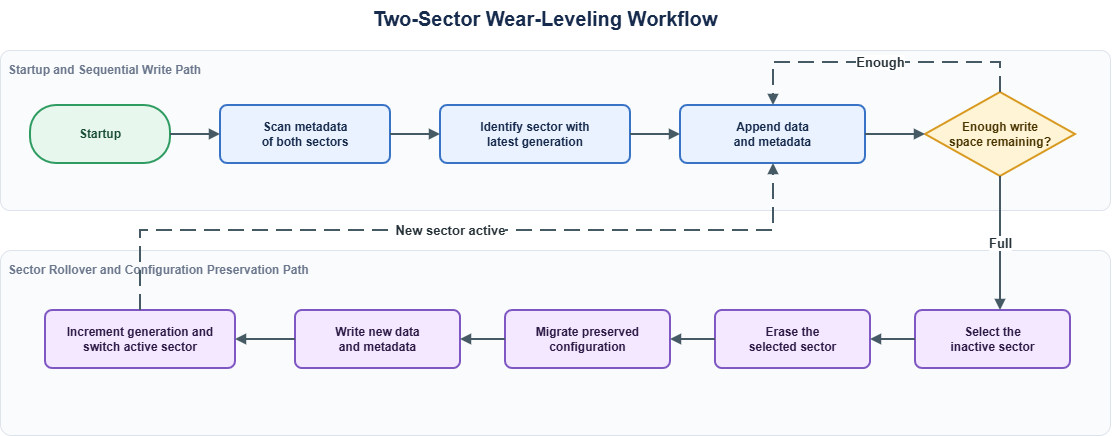
\includegraphics[width=6.5in,height=2.54861in]{media/image11.png}

\emph{Hình 3.x. Luồng xử lý khởi tạo, ghi nối tiếp và chuyển đổi
sector.}

Như trình bày trong Hình 3.y, khi khởi động, hệ thống quét metadata của
cả hai sector và lựa chọn sector chứa thế hệ hợp lệ mới nhất. Dữ liệu và
metadata tiếp tục được ghi nối tiếp cho đến khi không còn đủ không gian.
Khi đó, sector không hoạt động được xóa, cấu hình cần bảo toàn được
chuyển sang, sau đó dữ liệu mới được ghi và sector mới được đưa vào hoạt
động.

\textbf{Cấu trúc dữ liệu trong mỗi sector}

Mỗi sector được chia thành ba vùng có mục đích và phương thức cập nhật
khác nhau:

\begin{longtable}[]{@{}
  >{\raggedright\arraybackslash}p{(\columnwidth - 4\tabcolsep) * \real{0.1809}}
  >{\raggedright\arraybackslash}p{(\columnwidth - 4\tabcolsep) * \real{0.2910}}
  >{\raggedright\arraybackslash}p{(\columnwidth - 4\tabcolsep) * \real{0.5281}}@{}}
\toprule\noalign{}
\begin{minipage}[b]{\linewidth}\raggedright
\textbf{Thành phần}
\end{minipage} & \begin{minipage}[b]{\linewidth}\raggedright
\textbf{Phương thức cập nhật}
\end{minipage} & \begin{minipage}[b]{\linewidth}\raggedright
\textbf{Vai trò}
\end{minipage} \\
\midrule\noalign{}
\endhead
\bottomrule\noalign{}
\endlastfoot
Metadata & Ghi thêm mục mới & Mô tả vị trí, trạng thái và thứ tự của dữ
liệu \\
Configuration & Ghi ảnh cấu hình mới & Duy trì trạng thái vận hành gần
nhất \\
Log storage & Ghi nối tiếp bản ghi & Lưu lịch sử hoạt động và thông tin
chẩn đoán \\
\end{longtable}

\textbf{Tổ chức metadata}

Mỗi lần cấu hình hoặc nhật ký được ghi, hệ thống tạo một mục metadata
tương ứng. Thay vì chỉ đánh dấu vùng nhớ đã sử dụng, metadata cung cấp
đủ thông tin để hệ thống khôi phục trạng thái lưu trữ sau khi khởi động
lại.

\begin{longtable}[]{@{}
  >{\raggedright\arraybackslash}p{(\columnwidth - 2\tabcolsep) * \real{0.2975}}
  >{\raggedright\arraybackslash}p{(\columnwidth - 2\tabcolsep) * \real{0.7025}}@{}}
\toprule\noalign{}
\begin{minipage}[b]{\linewidth}\raggedright
\textbf{Nhóm thông tin}
\end{minipage} & \begin{minipage}[b]{\linewidth}\raggedright
\textbf{Mục đích}
\end{minipage} \\
\midrule\noalign{}
\endhead
\bottomrule\noalign{}
\endlastfoot
Marker và generation & Nhận dạng bản ghi hợp lệ và xác định thứ tự cập
nhật \\
Offset và kích thước & Xác định vị trí của dữ liệu trong sector \\
Timestamp & Ghi nhận thời điểm tạo bản ghi \\
CRC dữ liệu & Kiểm tra tính toàn vẹn của nội dung \\
CRC metadata & Phát hiện mục metadata bị ghi lỗi \\
Vị trí đọc nhật ký & Khôi phục phần nhật ký đã được tiếp nhận \\
\end{longtable}

Metadata được tổ chức theo phương pháp append-only. Khi có thay đổi, hệ
thống thêm một mục mới vào vị trí trống tiếp theo thay vì sửa mục đã tồn
tại. Cách làm này phù hợp với đặc tính của Flash: dữ liệu có thể được
lập trình vào vùng đã xóa, nhưng muốn ghi lại một vùng đã sử dụng phải
xóa toàn bộ sector.

Dữ liệu chính được ghi trước, metadata được thêm sau. Vì vậy, một vùng
dữ liệu chưa có metadata hợp lệ sẽ không được xem là bản ghi hoàn chỉnh.
Khi khởi động, hệ thống quét metadata, kiểm tra marker và CRC, sau đó
lựa chọn bản cấu hình có thứ tự cập nhật mới nhất.

\textbf{Lưu cấu hình và nhật ký}

Đối với cấu hình hệ thống, mỗi lần cập nhật tạo ra một ảnh cấu hình mới.
Các phiên bản cũ vẫn được giữ lại cho đến khi sector bị xóa. Khi cần
khôi phục, hệ thống lựa chọn bản mới nhất có metadata và CRC hợp lệ.

Nhật ký được ghi nối tiếp vào vùng log storage. Hệ thống duy trì vị trí
ghi hiện tại và vị trí mà máy chủ đã xác nhận đọc. Vị trí đọc được lưu
trong metadata, cho phép tiếp tục quá trình truyền nhật ký sau khi thiết
bị khởi động lại mà không phải quét toàn bộ dữ liệu để suy đoán trạng
thái.

\subsection{Chương trình khởi động nhúng}

\subsubsection{Quy trình xác thực và khởi chạy ứng dụng chính}

\begin{quote}
Sau mỗi lần cấp nguồn hoặc khởi động lại, vi điều khiển bắt đầu thực thi
tại vùng bootloader thay vì chuyển ngay đến chương trình ứng dụng.
Bootloader đóng vai trò là lớp trung gian có nhiệm vụ kiểm tra trạng
thái hệ thống, phát hiện yêu cầu bảo trì và chỉ chuyển quyền điều khiển
khi ảnh firmware trong vùng ứng dụng đáp ứng các điều kiện hợp lệ.

Trong giai đoạn đầu, bootloader khởi tạo các tài nguyên tối thiểu cần
thiết như hệ thống xung nhịp, giao tiếp USB, UART, BLE và cơ chế ghi
nhận trạng thái. Đồng thời, bootloader kiểm tra cờ yêu cầu nâng cấp được
ứng dụng lưu tạm trong RAM trước khi khởi động lại. Cờ này chỉ có hiệu
lực cho một lần khởi động và được xóa ngay sau khi đọc, nhờ đó thiết bị
không bị mắc kẹt trong chế độ bảo trì sau khi quá trình nâng cấp hoàn
tất.

Sau khi khởi tạo, bootloader mở một khoảng thời gian chờ để phát hiện
hoạt động từ công cụ cấu hình hoặc chương trình cập nhật firmware. Nếu
nhận được kết nối USB DFU, BLE FOTA hoặc yêu cầu nâng cấp chủ động từ
ứng dụng, thiết bị tiếp tục duy trì chế độ bootloader. Ngược lại, khi
hết thời gian chờ mà không có hoạt động bảo trì, bootloader bắt đầu xác
thực chương trình ứng dụng.

Quá trình xác thực trước khi khởi chạy tập trung vào hai nhóm điều kiện
chính:
\end{quote}

\begin{longtable}[]{@{}
  >{\raggedright\arraybackslash}p{(\columnwidth - 6\tabcolsep) * \real{0.1535}}
  >{\raggedright\arraybackslash}p{(\columnwidth - 6\tabcolsep) * \real{0.1444}}
  >{\raggedright\arraybackslash}p{(\columnwidth - 6\tabcolsep) * \real{0.3656}}
  >{\raggedright\arraybackslash}p{(\columnwidth - 6\tabcolsep) * \real{0.3366}}@{}}
\toprule\noalign{}
\begin{minipage}[b]{\linewidth}\raggedright
\textbf{Nhóm xác thực}
\end{minipage} & \begin{minipage}[b]{\linewidth}\raggedright
\textbf{Thành phần kiểm tra}
\end{minipage} & \begin{minipage}[b]{\linewidth}\raggedright
\textbf{Điều kiện hợp lệ}
\end{minipage} & \begin{minipage}[b]{\linewidth}\raggedright
\textbf{Mục đích}
\end{minipage} \\
\midrule\noalign{}
\endhead
\bottomrule\noalign{}
\endlastfoot
\textbf{Thông tin nhận dạng firmware} & Header Firmware Image & Giá trị
nhận dạng, phiên bản cấu trúc và kích thước tiêu đề phải phù hợp với
định dạng của hệ thống. & Phân biệt firmware hợp lệ với vùng nhớ trống,
dữ liệu chưa hoàn chỉnh hoặc ảnh không tương thích. \\
\textbf{Khả năng thực thi} & Bảng vector của ứng dụng & Con trỏ ngăn xếp
ban đầu phải nằm trong SRAM; địa chỉ hàm khởi động phải thuộc vùng nhớ
ứng dụng. & Bảo đảm bảng vector có cấu trúc hợp lệ và ứng dụng có thể
được CPU khởi chạy an toàn. \\
\end{longtable}

\begin{quote}
Đối với firmware vừa được nâng cấp, cần xác thực lại bằng cách tính CRC
của toàn bộ image sau đó so sánh với giá trị trong image header nhằm đảm
bảo ảnh nhận được là hợp lệ. Như vậy, hệ thống kết hợp kiểm tra cấu trúc
thực thi với kiểm tra tính toàn vẹn trong quá trình cài đặt firmware,
hạn chế việc khởi chạy một ảnh bị thiếu dữ liệu hoặc sai lệch trong quá
trình truyền.

Nếu chương trình ứng dụng không hợp lệ, bootloader không thực hiện
chuyển quyền mà tiếp tục duy trì chế độ bảo trì để chờ một ảnh firmware
mới. Cách xử lý này giúp thiết bị vẫn có khả năng phục hồi ngay cả khi
quá trình cập nhật trước đó bị gián đoạn.

Khi các điều kiện khởi chạy đã được đáp ứng, bootloader thực hiện quá
trình bàn giao có kiểm soát. Trước hết, các ngắt và bộ định thời hệ
thống được vô hiệu hóa; giao tiếp USB và các ngoại vi do bootloader sử
dụng được dừng; các cờ ngắt đang chờ cũng được xóa. Sau đó, địa chỉ bảng
vector được chuyển sang vùng ứng dụng, con trỏ ngăn xếp chính được nạp
từ bảng vector mới và CPU chuyển đến hàm khởi động của ứng dụng. Quy
trình này tạo cho chương trình chính một trạng thái khởi đầu độc lập,
tránh để cấu hình còn sót lại từ bootloader ảnh hưởng đến quá trình vận
hành.
\end{quote}

\subsubsection{Cơ chế nâng cấp và bảo trì hệ thống}

Hệ thống hỗ trợ nâng cấp firmware thông qua hai phương thức: cập nhật có
dây bằng USB DFU và cập nhật không dây bằng BLE FOTA. Cả hai phương thức
cùng sử dụng vùng nhớ ứng dụng đã được phân tách khỏi bootloader và vùng
dữ liệu vận hành. Việc phân vùng giúp quá trình ghi firmware không làm
thay đổi mã bootloader hoặc dữ liệu cấu hình được lưu giữ riêng.

Trong điều kiện vận hành bình thường, ứng dụng có thể chủ động yêu cầu
chuyển sang chế độ bảo trì. Khi nhận được lệnh hợp lệ, ứng dụng ghi một
cờ tạm vào RAM và thực hiện khởi động lại vi điều khiển. Bootloader đọc
cờ này trong lần khởi động tiếp theo, kéo dài thời gian chờ và duy trì
các giao tiếp cần thiết để công cụ nâng cấp kết nối với thiết bị. Cơ chế
này không yêu cầu ứng dụng tự ghi đè lên chính vùng mã đang thực thi.

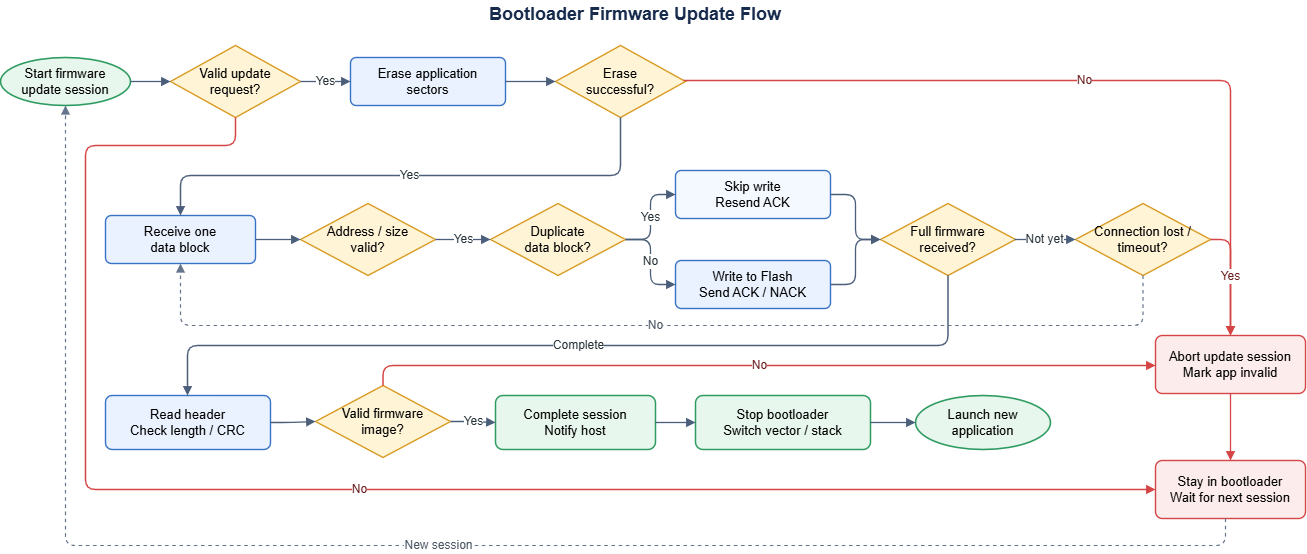
\includegraphics[width=6.77708in,height=2.87409in]{media/image12.png}

\subsection{Kiến trúc phần mềm ứng dụng đa nhiệm}

\subsubsection{Kiến trúc phân tầng phần mềm ứng dụng}

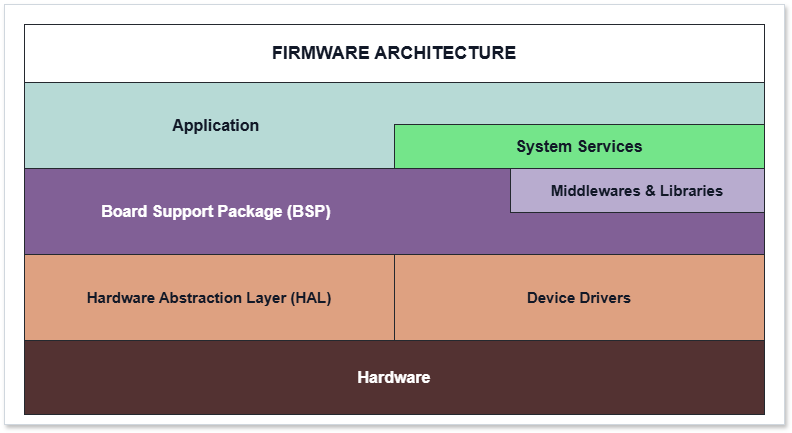
\includegraphics[width=3.82143in,height=2.08995in]{media/image13.png}

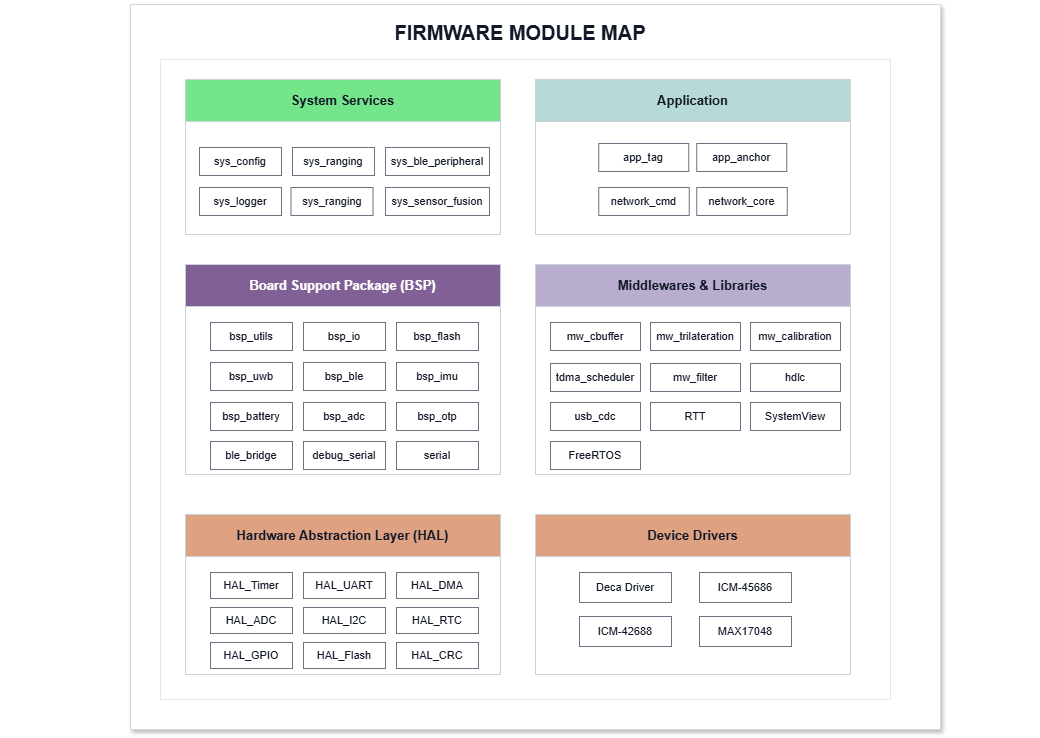
\includegraphics[width=6.5in,height=4.61528in]{media/image14.png}

\subsubsection{Quản lý đa nhiệm và đồng bộ hóa tài nguyên với freeRTOSx}

Firmware được tổ chức theo mô hình đa nhiệm ưu tiên trên. Mục tiêu của
kiến trúc là tách luồng định vị UWB có yêu cầu thời gian thực khỏi các
tác vụ tính toán, truyền thông, giám sát và lưu trữ nền. Trên vi điều
khiển đơn lõi, các tác vụ không thực thi song song mà được scheduler
chuyển đổi theo trạng thái sẵn sàng và mức ưu tiên.

Scheduler sử dụng cơ chế cưỡng đoạt: khi một tác vụ ưu tiên cao được
đánh thức bởi ngắt hoặc sự kiện, tác vụ này có thể chiếm quyền xử lý từ
tác vụ ưu tiên thấp hơn. Ngược lại, semaphore, queue và các lệnh delay
đưa tác vụ về trạng thái chờ, nhờ đó CPU được dành cho workflow đang có
dữ liệu cần xử lý.

\textbf{a) Tổ chức tác vụ và phân cấp ưu tiên}

Các tác vụ được phân chia theo vai trò chức năng và độ khẩn cấp của dữ
liệu. UwbRanging giữ mức ưu tiên cao nhất để đáp ứng các mốc thời gian
của giao thức ranging; SensorFusion xử lý dữ liệu định vị ở mức ưu tiên
kế tiếp; các tác vụ dịch vụ được chạy khi luồng thời gian thực đang chờ
sự kiện.

\begin{longtable}[]{@{}
  >{\raggedright\arraybackslash}p{(\columnwidth - 6\tabcolsep) * \real{0.1769}}
  >{\raggedright\arraybackslash}p{(\columnwidth - 6\tabcolsep) * \real{0.1684}}
  >{\raggedright\arraybackslash}p{(\columnwidth - 6\tabcolsep) * \real{0.2470}}
  >{\raggedright\arraybackslash}p{(\columnwidth - 6\tabcolsep) * \real{0.4077}}@{}}
\toprule\noalign{}
\begin{minipage}[b]{\linewidth}\raggedright
\textbf{Tác vụ}
\end{minipage} & \begin{minipage}[b]{\linewidth}\raggedright
\textbf{Ưu tiên}
\end{minipage} & \begin{minipage}[b]{\linewidth}\raggedright
\textbf{Cơ chế kích hoạt}
\end{minipage} & \begin{minipage}[b]{\linewidth}\raggedright
\textbf{Chức năng chính}
\end{minipage} \\
\midrule\noalign{}
\endhead
\bottomrule\noalign{}
\endlastfoot
\textbf{UwbRanging} & Realtime & Semaphore UWB hoặc timeout động & Xử lý
DW1000 và state machine của Tag/Anchor \\
\textbf{SensorFusion} & High & Chu kỳ 20 ms và dữ liệu từ queue & IMU
predict, lọc khoảng cách, trilateration và UKF update \\
\textbf{Network} & Normal & Định kỳ 5 ms & Xử lý giao tiếp UART, USB và
BLE \\
\textbf{SysMonitoring} & BelowNormal & Định kỳ 30 s & Theo dõi mức sử
dụng stack, heap và CPU \\
\textbf{FlashStorage} & Low & Định kỳ 2 s & Ghi dữ liệu log từ RAM xuống
bộ nhớ Flash \\
\textbf{PM} & Low & Định kỳ 100 ms & Giám sát nhiệt độ, mức điện áp, pin
và xử lý lỗi phần cứng nhằm đảm bảo bo mạch được đưa về trạng thái an
toàn \\
\textbf{IO} & Low & Semaphore nút nhấn và timeout 100 ms & Xử lý nút
nhấn, LED và các ngoại vi trên board \\
\end{longtable}

\emph{Hình 3.x. Kiến trúc thực thi và đồng bộ hóa tài nguyên bằng
FreeRTOS.}

\textbf{b) Quy trình khởi tạo và vận hành của hệ điều hành}

Workflow của hệ điều hành được chia thành pha khởi tạo trước kernel và
pha vận hành sau khi scheduler được kích hoạt. Chuỗi thực thi chính được
mô tả như sau:

\textbf{c) Cơ chế đồng bộ hóa và bảo vệ tài nguyên}

Semaphore: được sử dụng để truyền sự kiện từ ISR sang tác vụ.
g\_uwb\_isr\_semHandle đánh thức UwbRanging khi có sự kiện DW1000, trong
khi g\_io\_btn\_semHandle chuyển sự kiện nút nhấn sang IO. Cơ chế này
giữ ISR ngắn và chuyển phần xử lý dài vào bên trong tác vụ.

Mutex: được sử dụng để bảo vệ tài nguyên dùng chung.
g\_spi1\_mutexHandle tuần tự hóa truy cập bus SPI1 giữa DW1000, IMU và
các lần đọc telemetry của PM; g\_logger\_mutexHandle bảo vệ vùng log
vòng trong RAM. Mutex chỉ được giữ trong khoảng thời gian cần thiết để
hạn chế blocking đối với tác vụ ưu tiên cao.

Message queue: được sử dụng để truyền dữ liệu có cấu trúc giữa các tác
vụ. g\_uwb\_distance\_queue tách thời điểm thu thập khoảng cách trong
UwbRanging khỏi thời điểm xử lý thuật toán trong SensorFusion, nhờ đó
hai task không phải chia sẻ trực tiếp một vùng dữ liệu thay đổi đồng
thời.

Logging: được tổ chức thành side path độc lập. Các tác vụ ghi bản ghi
qua RLOG\_* vào RAM circular buffer; FlashStorage định kỳ chuyển dữ liệu
xuống Flash. Vì đường log không nằm trên chuỗi định vị chính, độ trễ ghi
Flash không chặn workflow UWB.

\subsection{Triển khai các thuật toán định vị nhúng}

Chuỗi xử lý định vị được trình bày theo thứ tự của dữ liệu. Trước hết, kiến
trúc tầng xử lý xác định luồng trao đổi giữa các khối; tiếp theo, DS--TWR,
TDMA và CDMA tổ chức quá trình thu thập range. Prefilter thống kê sau đó xây
dựng measurement weight và lựa chọn layout bằng WGDOP. Cùng một tập range,
trọng số và layout sau prefilter được đưa song song vào WLS multilateration và
UKF để so sánh. Cách tổ chức này tách rõ bốn vấn đề: thu thập dữ liệu, đánh
giá phép đo, đánh giá hình học và lựa chọn phương pháp ước lượng vị trí.

\subsubsection{Kiến trúc tầng xử lý dữ liệu định vị}

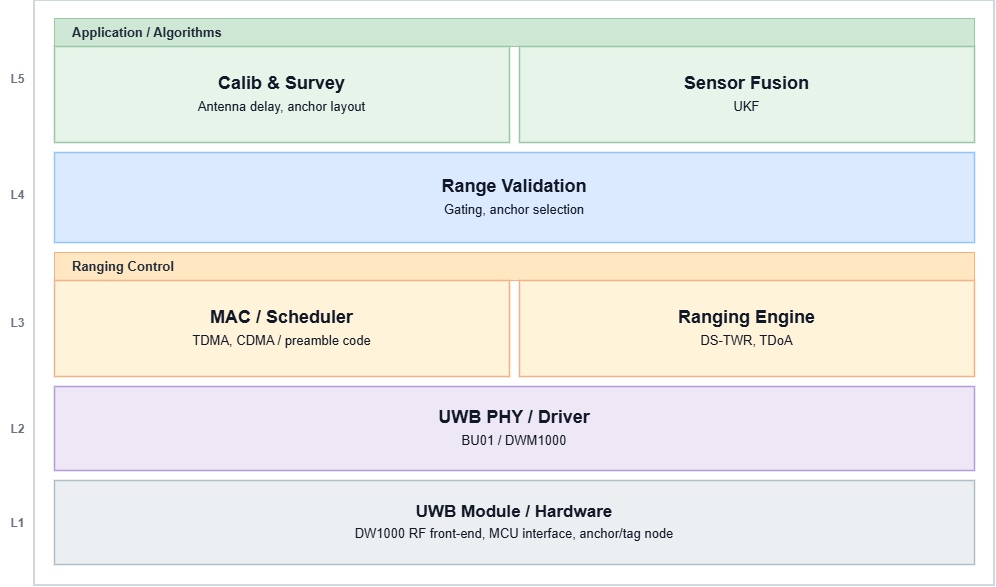
\includegraphics[width=6.5in,height=3.83264in]{media/image15.png}

\subsubsection{Thuật toán đo khoảng cách và bộ lập lịch}

Đầu vào của thuật toán định vị không chỉ phụ thuộc vào độ chính xác của phép đo
khoảng cách, mà còn phụ thuộc vào việc các phép đo có được thu nhận trong cùng
một chu kỳ và không bị xung đột trên kênh truyền hay không. Vì vậy, khối thu
thập dữ liệu được thiết kế như một chuỗi thống nhất gồm ba chức năng: DS--TWR
thực hiện phép đo khoảng cách, TDMA xác lập trật tự truy nhập kênh trong một
vùng, còn preamble code hỗ trợ phân tách các vùng UWB lân cận. Ba chức năng này
không thay thế lẫn nhau mà giải quyết ba lớp vấn đề khác nhau, như tóm tắt trong
Bảng~\ref{tab:ranging-scheduler-layers}.

\begin{longtable}{@{}p{0.19\textwidth}p{0.25\textwidth}p{0.45\textwidth}@{}}
\caption{Vai trò của các lớp trong quá trình thu thập range.}
\label{tab:ranging-scheduler-layers}\\
\toprule
\textbf{Lớp} & \textbf{Phạm vi} & \textbf{Chức năng} \\
\midrule
\endfirsthead
\toprule
\textbf{Lớp} & \textbf{Phạm vi} & \textbf{Chức năng} \\
\midrule
\endhead
DS--TWR & Một liên kết tag--anchor & Ước lượng thời gian truyền và khoảng cách \\
TDMA & Các anchor trong cùng vùng & Ấn định thứ tự và thời điểm phát RESP \\
Preamble code & Các vùng UWB lân cận & Phân biệt nhóm thiết bị ở tầng vật lý \\
\bottomrule
\end{longtable}

\textbf{Tổ chức một chu kỳ đo.} Tag khởi tạo chu kỳ bằng gói POLL dùng chung
cho nhóm anchor đang hoạt động. Sau khi nhận POLL, mỗi anchor chỉ phát RESP tại
khe thời gian đã được gán. Tag thu các phản hồi trong một cửa sổ xác định rồi
phát FINAL chứa các mốc thời gian cần thiết cho phép tính DS--TWR. Cuối cùng,
từng anchor hoàn tất phép tính thời gian truyền và gửi RESULT về tag. Trình tự
POLL--RESP--FINAL--RESULT tạo ra một tập range có chung chỉ số chu kỳ; nhờ đó,
tầng định vị có thể xem các range hợp lệ như các quan sát gần đồng thời thay vì
tập hợp những phép đo rời rạc.

\textbf{Quy tắc lập lịch TDMA.} Nếu anchor $i$ được gán chỉ số khe $s_i$, thời
điểm phát RESP dự kiến được xác định bởi

\begin{equation}
  t_{\mathrm{RESP},i}=t_{\mathrm{POLL}}+T_{\mathrm{offset}}
  +s_iT_{\mathrm{slot}},
  \label{eq:tdma-response-time}
\end{equation}
trong đó $T_{\mathrm{offset}}$ là thời gian từ lúc phát POLL đến đầu cửa sổ
RESP và $T_{\mathrm{slot}}$ là độ dài một khe. Để hai phản hồi liên tiếp không
chồng lấn, độ dài khe phải thỏa mãn
\begin{equation}
  T_{\mathrm{slot}}\geq
  T_{\mathrm{frame}}+T_{\mathrm{proc}}+T_{\mathrm{guard}},
  \label{eq:tdma-slot-condition}
\end{equation}
trong đó $T_{\mathrm{frame}}$ là thời gian truyền RESP,
$T_{\mathrm{proc}}$ là thời gian xử lý cần thiết và $T_{\mathrm{guard}}$ là
biên dự phòng cho sai lệch đồng hồ cũng như jitter. Các mốc phát yêu cầu độ
chính xác cao được ràng buộc theo đồng hồ UWB; bộ lập lịch mức hệ thống chỉ quản
lý trạng thái của chu kỳ và các sự kiện hoàn thành.

\textbf{Khả năng mở rộng và xử lý mất gói.} Với $N_{\mathrm{anchor}}$ anchor,
thời gian của một chu kỳ có thể xấp xỉ bởi
\begin{equation}
  T_{\mathrm{sf}}\approx T_{\mathrm{fixed}}+
  N_{\mathrm{anchor}}T_{\mathrm{slot}},
  \label{eq:tdma-superframe-duration}
\end{equation}
trong đó $T_{\mathrm{fixed}}$ bao gồm các pha POLL, FINAL, RESULT và khoảng bảo
vệ chung. Biểu thức cho thấy tốc độ cập nhật giảm gần tuyến tính khi số anchor
tăng; vì vậy số anchor tham gia, độ dài khe và tần số định vị phải được lựa chọn
đồng thời. Nếu một anchor không phản hồi, khe của anchor đó không được dồn hoặc
chuyển sang vị trí khác trong chính chu kỳ đang xét. Chu kỳ vẫn tiếp tục theo
lịch ban đầu, còn range tương ứng được đánh dấu không hợp lệ. Quy tắc này giữ
cấu trúc thời gian có tính xác định và ngăn một lỗi cục bộ làm sai lệch thời
điểm của các anchor phía sau. Tập dữ liệu chỉ được chuyển sang bước định vị khi
số range hợp lệ đáp ứng điều kiện quan sát tối thiểu.

\textbf{Phân tách nhiều vùng bằng mã.} TDMA giải quyết tranh chấp giữa các
anchor dùng chung một vùng, nhưng không tự phân biệt các mạng UWB lân cận. Mỗi
vùng vì vậy được liên kết với một preamble code, một danh sách anchor và một
ánh xạ khe riêng. Xét theo nguyên lý đa truy nhập, cách tổ chức này bổ sung một
chiều phân tách theo mã tương tự CDMA: bộ thu ưu tiên phát hiện chuỗi preamble
đã cấu hình, trong khi TDMA vẫn quyết định thời điểm truyền trong nội vùng.
Tuy nhiên, preamble code không được xem là cơ chế cách ly tuyệt đối; mức độ
giao thoa giữa các mã vẫn phụ thuộc cấu hình PHY và điều kiện triển khai thực
tế.

Khi tag chuyển vùng, ba thành phần gồm preamble code, tập anchor và ánh xạ khe
phải được cập nhật như một cấu hình thống nhất. Chu kỳ hiện tại được kết thúc
trước khi cấu hình mới có hiệu lực; các mốc thời gian thuộc vùng cũ không được
tái sử dụng cho chu kỳ tiếp theo. Nhờ đó, một tập range luôn thuộc về duy nhất
một vùng và một cấu hình lập lịch, bảo đảm tính nhất quán cho dữ liệu đưa vào
prefilter và thuật toán định vị.

\subsubsection{Các hướng tiếp cận thuật toán định vị từ dữ liệu UWB}

Từ dữ liệu khoảng cách UWB, bài toán định vị có thể được triển khai theo hai
hướng chính. Hướng thứ nhất giải trực tiếp bài toán hình học tại từng chu kỳ
đo, không duy trì trạng thái động học giữa các chu kỳ. Hướng thứ hai sử dụng
bộ ước lượng trạng thái để khai thác tính liên tục của chuyển động và kết hợp
thông tin từ nhiều thời điểm.

Trong đề tài, prefilter là tầng dùng chung cho cả hai hướng. Tầng này đánh giá
độ tin cậy của từng range, xây dựng measurement weight và lựa chọn layout
anchor. Đầu ra của prefilter được giữ giống nhau khi đưa vào hai bộ ước lượng:
WLS multilateration giải nghiệm hình học độc lập tại mỗi chu kỳ, còn UKF ước
lượng trạng thái đệ quy dựa trên mô hình chuyển động. Nhờ đó, chênh lệch kết
quả phản ánh phương pháp ước lượng thay vì khác biệt ở bước xử lý đầu vào.

\begin{longtable}{@{}p{0.20\textwidth}p{0.33\textwidth}p{0.35\textwidth}@{}}
\caption{So sánh sơ bộ hai phương án định vị.}
\label{tab:wls-ukf-comparison}\\
\toprule
\textbf{Tiêu chí} & \textbf{WLS multilateration} &
\textbf{UKF} \\
\midrule
\endfirsthead
\toprule
\textbf{Tiêu chí} & \textbf{WLS multilateration} &
\textbf{UKF} \\
\midrule
\endhead
Đầu vào & Range, weight và layout sau prefilter &
Range, weight và layout sau prefilter \\
Nguyên lý ước lượng & Tối ưu phi tuyến tại từng chu kỳ &
Ước lượng trạng thái đệ quy \\
Thông tin thời gian & Không duy trì trạng thái động học &
Khai thác trạng thái và covariance chu kỳ trước \\
Đầu ra & Vị trí tại thời điểm hiện tại &
Trạng thái vị trí, vận tốc và độ bất định \\
Mất quan sát ngắn hạn & Không tạo nghiệm mới từ dự đoán &
Có thể duy trì bước dự đoán \\
Chi phí tính toán & Thấp đến trung bình &
Cao hơn do lan truyền và cập nhật trạng thái \\
\bottomrule
\end{longtable}

Hai phương pháp được đánh giá trên cùng log dữ liệu, tọa độ anchor, mốc thời
gian và đầu ra prefilter. Các chỉ tiêu gồm sai số vị trí, độ ổn định quỹ đạo,
tỷ lệ tạo được nghiệm và thời gian xử lý. Việc giữ nguyên đầu vào cho phép
đánh giá riêng lợi ích của ước lượng trạng thái theo thời gian so với nghiệm
hình học độc lập.

\subsubsection{WLS multilateration}

Gọi $\mathbf p=[x\;y]^T$ là vị trí cần xác định,
$\mathbf a_i=[x_i\;y_i]^T$ là tọa độ anchor thứ $i$ và $d_i$ là range đo
được. Khoảng cách dự đoán và residual tương ứng là
\begin{align}
  \widehat d_i(\mathbf p)&=
  \lVert\mathbf p-\mathbf a_i\rVert,\\
  r_i(\mathbf p)&=d_i-\widehat d_i(\mathbf p).
  \label{eq:wls-range-residual}
\end{align}
Với tập anchor hợp lệ $\mathcal A$, nghiệm WLS được xác định bởi
\begin{equation}
  \widehat{\mathbf p}_{\mathrm{WLS}}=
  \arg\min_{\mathbf p}
  \frac{1}{2}\mathbf r^T\mathbf W\mathbf r
  =\arg\min_{\mathbf p}
  \sum_{i\in\mathcal A}w_i r_i^2(\mathbf p),
  \label{eq:wls-objective-detailed}
\end{equation}
trong đó $\mathbf W=\operatorname{diag}(w_1,\ldots,w_N)$ là ma trận trọng
số. Khi chỉ biết mô hình phương sai, lựa chọn cơ bản là
$w_i\propto 1/\sigma_r^2(d_i)$; các hệ số chất lượng từ prefilter có thể được
kết hợp vào inverse-variance weight này.

Do mô hình range phi tuyến theo $\mathbf p$, nghiệm được tìm lặp bằng
Gauss--Newton. Tại nghiệm tạm $\mathbf p^{(t)}$, hàng thứ $i$ của Jacobian là
\begin{equation}
  \mathbf J_i=
  \begin{bmatrix}
  \dfrac{x^{(t)}-x_i}{\widehat d_i} &
  \dfrac{y^{(t)}-y_i}{\widehat d_i}
  \end{bmatrix},
  \label{eq:wls-jacobian}
\end{equation}
và bước hiệu chỉnh được tính bởi
\begin{equation}
  \Delta\mathbf p=
  (\mathbf J^T\mathbf W\mathbf J)^{-1}
  \mathbf J^T\mathbf W\mathbf r,
  \qquad
  \mathbf p^{(t+1)}=\mathbf p^{(t)}+\Delta\mathbf p.
  \label{eq:wls-gauss-newton}
\end{equation}

Giá trị khởi tạo có thể lấy từ nghiệm tuyến tính, trọng tâm của tập anchor
hoặc nghiệm chu kỳ trước. Quá trình lặp dừng khi
$\lVert\Delta\mathbf p\rVert$ nhỏ hơn ngưỡng hội tụ hoặc đạt số vòng lặp tối
đa. Nghiệm không được sử dụng khi số anchor không đủ, ma trận
$\mathbf J^T\mathbf W\mathbf J$ kém điều kiện hoặc residual sau hội tụ vượt
giới hạn chấp nhận.

\subsubsection{Prefilter thống kê và xây dựng measurement weight}

Các phép đo UWB chịu ảnh hưởng đồng thời của nhiễu ngẫu nhiên, sai lệch NLOS
và cấu hình hình học anchor. Ba yếu tố này có bản chất khác nhau: nhiễu đo làm
tăng phương sai của range, NLOS tạo sai lệch có hướng, còn hình học kém khuếch
đại sai số range thành sai số vị trí. Vì vậy, prefilter không nên quy đổi trực
tiếp mọi đại lượng thành các điểm số độc lập rồi cộng lại. Trong đề tài, chất
lượng phép đo được mô tả trước bằng độ chính xác tương đối của từng anchor;
thông tin hình học chỉ được đưa vào sau thông qua ma trận thông tin của layout.

Mô hình range của anchor thứ $i$ được viết dưới dạng
\begin{equation}
  d_i=h_i(\mathbf{x})+b_i+\varepsilon_i,
  \qquad
  h_i(\mathbf{x})=\lVert\mathbf{p}-\mathbf{a}_i\rVert,
  \label{eq:prefilter-range-model}
\end{equation}
trong đó $\varepsilon_i$ là nhiễu ngẫu nhiên có kỳ vọng xấp xỉ bằng 0 và
$b_i$ là thành phần bias. Trong điều kiện LOS, $b_i$ thường nhỏ; khi đường
truyền bị che khuất, $b_i$ có thể tăng đáng kể và làm range lệch về phía
dương. Prefilter có nhiệm vụ phát hiện các phép đo không nhất quán, giảm ảnh
hưởng của những phép đo đáng ngờ và duy trì đủ thông tin để ước lượng vị trí.

\paragraph{Kiểm tra nhất quán bằng Mahalanobis distance.}

Từ trạng thái dự đoán $\widehat{\mathbf{x}}^{-}$, khoảng cách dự đoán và
innovation của phép đo được xác định bởi
\begin{align}
  \widehat d_i^{-}&=h_i(\widehat{\mathbf{x}}^{-}),\\
  \nu_i&=d_i-\widehat d_i^{-}.
  \label{eq:prefilter-range-innovation}
\end{align}
Gọi $S_i$ là phương sai innovation, bao gồm bất định của trạng thái dự đoán
và phương sai của phép đo range. Mahalanobis distance squared là
\begin{equation}
  D_i^2=\frac{\nu_i^2}{S_i}.
  \label{eq:prefilter-mahalanobis}
\end{equation}
Nếu innovation tuân theo phân bố Gaussian và mô hình được xác định đúng,
$D_i^2$ xấp xỉ phân bố $\chi^2$ với một bậc tự do. Do đó, ngưỡng loại ngoại
lai có thể được lựa chọn từ phân vị của phân bố $\chi_1^2$ ứng với mức tin cậy
mong muốn. Hai ngưỡng khác nhau được sử dụng cho quá trình loại và phục hồi
phép đo nhằm tạo hysteresis, tránh thay đổi quyết định liên tục khi
$D_i^2$ dao động gần biên.

Ngoài quyết định gate, Mahalanobis distance còn được sử dụng như một
độ lệch chuẩn hóa của phép đo:
\begin{equation}
  u_i^{\mathrm{M}}=\sqrt{D_i^2}.
  \label{eq:mahalanobis-standardized-deviation}
\end{equation}
Giá trị này được chuyển thành trọng số mềm cùng với FP amplitude và residual
bằng một hàm ảnh hưởng thống nhất được trình bày ở phần sau.

\paragraph{Đánh giá đường truyền bằng FP amplitude.}

FP amplitude mô tả biên độ tín hiệu tại vùng lân cận thời điểm phát hiện đường
truyền đầu tiên. Với ba mẫu biên độ $A_{1,i}$, $A_{2,i}$ và $A_{3,i}$ cùng số
xung preamble được tích lũy $N_{\mathrm{pacc},i}$, đại lượng sử dụng trong
prefilter được xác định bởi
\begin{equation}
  A_{\mathrm{FP},i}=
  \frac{A_{1,i}+A_{2,i}+A_{3,i}}{N_{\mathrm{pacc},i}}.
  \label{eq:first-path-amplitude}
\end{equation}
Đây là đại lượng chẩn đoán biên độ của bộ thu, không phải công suất thu theo
dBm. Giá trị của nó phụ thuộc vào khoảng cách, cấu hình PHY, anten và môi
trường truyền; vì vậy một ngưỡng biên độ cố định không đủ để phân biệt LOS và
NLOS.

Để loại ảnh hưởng suy hao theo khoảng cách, FP amplitude được đưa về miền
logarithm
\begin{equation}
  a_i=20\log_{10}(A_{\mathrm{FP},i}+\varepsilon),
  \label{eq:fp-amplitude-log-domain}
\end{equation}
và so sánh với mô hình LOS đã hiệu chuẩn. Gọi $\mu_A(d)$ và $\sigma_A(d)$ lần
lượt là giá trị trung bình và độ lệch chuẩn của $a_i$ tại khoảng cách $d$ trong
điều kiện LOS, chỉ số chuẩn hóa là
\begin{equation}
  z_i^{A}=\frac{a_i-\mu_A(d_i)}{\sigma_A(d_i)+\varepsilon}.
  \label{eq:fp-amplitude-standard-score}
\end{equation}
Độ suy giảm bất thường của first path được biểu diễn bằng sai lệch một
phía
\begin{equation}
  u_i^{\mathrm{A}}=
  \max\!\left(0,
  \frac{\mu_A(d_i)-a_i}{\sigma_A(d_i)+\varepsilon}\right).
  \label{eq:fp-amplitude-standardized-deviation}
\end{equation}
Giá trị bằng 0 cho biết FP amplitude không thấp hơn mức LOS kỳ vọng; giá trị
dương cho biết mức thiếu hụt biên độ tính theo số độ lệch chuẩn. Cách định
nghĩa một phía phù hợp hơn trị tuyệt đối vì biên độ thấp bất thường mới là dấu
hiệu cần giảm trọng số, trong khi biên độ cao không được xem là ngoại lai xấu.

\paragraph{Trọng số bền vững từ residual.}

Sau bước gate, một nghiệm sơ bộ $\widehat{\mathbf p}^{(0)}$ được tính từ các
phép đo còn lại. Residual hình học của anchor thứ $i$ là
\begin{equation}
  e_i=d_i-
  \left\lVert\widehat{\mathbf p}^{(0)}-\mathbf a_i\right\rVert.
  \label{eq:prefilter-geometric-residual}
\end{equation}
Độ phân tán của residual được ước lượng bền vững bằng median absolute
deviation (MAD):
\begin{equation}
  s_e=1.4826\,
  \operatorname{median}_i
  \left|e_i-\operatorname{median}_j(e_j)\right|+\varepsilon.
  \label{eq:residual-robust-scale}
\end{equation}
Residual được đưa về độ lệch chuẩn hóa bền vững
\begin{equation}
  u_i^{\mathrm{R}}=
  \frac{\left|e_i-\operatorname{median}_j(e_j)\right|}{s_e}.
  \label{eq:residual-standardized-deviation}
\end{equation}

\paragraph{Hàm trọng số bền vững thống nhất.}

Ba đại lượng $u_i^{\mathrm{M}}$, $u_i^{\mathrm{A}}$ và
$u_i^{\mathrm{R}}$ đều là độ lệch không thứ nguyên, trong đó giá trị lớn biểu
thị phép đo kém tin cậy. Thay vì xây dựng ba công thức penalty riêng biệt, đề
tài sử dụng cùng một hàm trọng số Huber
\begin{equation}
  q(u;c)=
  \begin{cases}
    1, & |u|\leq c,\\
    \dfrac{c}{|u|+\varepsilon}, & |u|>c.
  \end{cases}
  \label{eq:unified-huber-weight}
\end{equation}
Các trọng số thành phần được viết gọn dưới dạng
\begin{equation}
  q_i^{\mathrm{M}}=q(u_i^{\mathrm{M}};c_{\mathrm{M}}),\qquad
  q_i^{\mathrm{A}}=q(u_i^{\mathrm{A}};c_{\mathrm{A}}),\qquad
  q_i^{\mathrm{R}}=q(u_i^{\mathrm{R}};c_{\mathrm{R}}).
  \label{eq:component-huber-weights}
\end{equation}
Các hằng số $c_{\mathrm{M}}$, $c_{\mathrm{A}}$ và $c_{\mathrm{R}}$ cho phép
điều chỉnh độ nhạy của từng nguồn thông tin nhưng không làm thay đổi dạng hàm.
Huber được lựa chọn vì hàm mất mát lồi, giảm ảnh hưởng ngoại lai một cách liên
tục và không đặt trọng số bằng 0. Các ngoại lai nghiêm trọng đã được xử lý bởi
Mahalanobis gate, do đó không cần thêm một cơ chế loại cứng ở tầng residual.

\paragraph{Ảnh hưởng của khoảng cách đo.}

Khoảng cách không được xem là một dấu hiệu ngoại lai, bởi một phép đo xa vẫn
có thể hoàn toàn hợp lệ. Tuy nhiên, phương sai range thường tăng theo khoảng
cách do suy hao tín hiệu và xác suất che khuất lớn hơn. Ảnh hưởng này được mô
tả trực tiếp bằng hàm phương sai phụ thuộc khoảng cách
\begin{equation}
  \sigma_r^2(d)=
  \mathbb{E}\!\left[(d_{\mathrm{meas}}-d_{\mathrm{ref}})^2
  \mid d,\mathrm{LOS}\right],
  \label{eq:distance-dependent-range-variance}
\end{equation}
được ước lượng từ dữ liệu hiệu chuẩn LOS theo từng khoảng cách hoặc từng bin.
Như vậy, distance tham gia measurement weight thông qua inverse variance;
phép đo xa có phương sai lớn hơn và tự động nhận trọng số thấp hơn. Cách xử lý
này tránh đưa distance qua Huber hoặc nhân thêm một penalty tùy ý, đồng thời
tránh đếm lặp ảnh hưởng suy hao đã được bù trong FP amplitude.

\paragraph{Xây dựng measurement weight.}

Mahalanobis distance, FP amplitude và residual lần lượt phản ánh tính nhất
quán theo thời gian, chất lượng đường truyền và tính nhất quán hình học trong
frame hiện tại. Sau khi được đưa qua cùng hàm Huber, chúng được hợp nhất thành
precision weight của phép đo:
\begin{equation}
  \widetilde w_i^{\mathrm{meas}}=
  \frac{q_i^{\mathrm{M}}q_i^{\mathrm{A}}q_i^{\mathrm{R}}}
       {\sigma_r^{2}(d_i)+\varepsilon},
  \label{eq:measurement-precision-weight}
\end{equation}
Biểu thức tích bảo đảm một phép đo chỉ nhận trọng số cao khi đồng thời phù hợp
với dự đoán, có first path đáng tin cậy, nhất quán với các phép đo còn lại và
có phương sai phù hợp với khoảng cách hiện tại. Khi giải WLS,
trọng số được chuẩn hóa trong layout:
\begin{equation}
  w_i^{\mathrm{meas}}=
  \frac{\widetilde w_i^{\mathrm{meas}}}
       {\sum_{j\in\mathcal L}\widetilde w_j^{\mathrm{meas}}}.
  \label{eq:normalized-measurement-weight}
\end{equation}
Phép chuẩn hóa này không làm thay đổi nghiệm WLS; các precision weight chưa
chuẩn hóa vẫn được giữ để xây dựng ma trận thông tin của layout.

\subsubsection{Lựa chọn layout anchor bằng WGDOP}

GDOP thông thường giả thiết mọi phép đo có cùng phương sai. Giả thiết này
không còn phù hợp khi từng anchor đã có measurement weight khác nhau. Vì vậy,
đề tài sử dụng dạng GDOP có trọng số. Với $\mathbf H_{\mathcal L}$ là ma trận
hình học của layout $\mathcal L$ và
$\mathbf{W}_{\mathcal L}=\operatorname{diag}
(\widetilde w_i^{\mathrm{meas}})$, ma trận thông tin vị trí là
\begin{equation}
  \mathbf I_{\mathcal L}=
  \mathbf H_{\mathcal L}^{T}
  \mathbf W_{\mathcal L}
  \mathbf H_{\mathcal L}.
  \label{eq:weighted-layout-information}
\end{equation}
Hiệp phương sai vị trí xấp xỉ được xác định bởi
\begin{equation}
  \mathbf C_{\mathbf p,\mathcal L}
  \approx \mathbf I_{\mathcal L}^{-1},
  \label{eq:layout-position-covariance}
\end{equation}
và tiêu chí lựa chọn layout là
\begin{equation}
  \operatorname{WGDOP}(\mathcal L)=
  \sqrt{\operatorname{tr}
  \left(\mathbf C_{\mathbf p,\mathcal L}\right)}.
  \label{eq:weighted-gdop}
\end{equation}
Layout có WGDOP nhỏ nhất được ưu tiên. Công thức này hợp nhất chất lượng phép
đo và hình học trong một đại lượng duy nhất: measurement weight xác định độ
tin cậy của từng hướng đo, còn $\mathbf H_{\mathcal L}$ xác định mức quan sát
được theo không gian. Nhờ đó không cần chuẩn hóa GDOP và các chỉ số chất lượng
về cùng miền rồi cộng bằng các hệ số tùy ý.

Để tránh thay đổi layout liên tục khi nhiều ứng viên có WGDOP gần tương
đương, layout của chu kỳ trước được giữ lại nếu mức cải thiện của ứng viên mới
chưa vượt quá một switch margin. Quy tắc này chỉ tạo hysteresis cho quyết định
lựa chọn layout và không làm thay đổi measurement weight đã ước lượng.

\subsubsection{Thuật toán sensor fusion với UKF}

% Phần logic UKF được bổ sung độc lập.
\vspace{4cm}

\subsubsection{Thuật toán hiệu chuẩn antenna delay và đo đạc vị trí anchor}

\subsection{Các dịch vụ hệ thống và quản trị thiết bị}

\section{Chương trình khối truyền thông không dây BLE}

\subsection{Cấu hình BLE trên SoC NRF52}

\subsection{Giao thức đóng gói và định tuyến dữ liệu}

\section{Thiết kế và triển khai chương trình giám sát trên máy tính}

\subsection{Kiến trúc tổng thể của phần mềm}

\subsection{Luồng xử lý của hệ thống}

\subsection{Thiết kế đa luồng và cơ chế đồng bộ dữ liệu}

\begin{quote}
\chapter{KẾT QUẢ THỰC NGHIỆM VÀ ĐÁNH GIÁ}
\end{quote}

\section{Kiểm chứng phần cứng và nguồn cấp}

\section{Đánh giá tài nguyên xử lý và khả năng đáp ứng định vị thời gian thực}

\section{Mô phỏng thuật toán định vị}

\section{Thực nghiệm định vị trong nhiều môi trường}

\section{Đánh giá cơ chế phân vùng không gian bằng CDMA}

\section{Tổng hợp và nhận xét kết quả thực nghiệm}

\end{document}
